\documentclass[12pt]{article}

\usepackage{sbc-template}
\usepackage{graphicx,url}
\usepackage[utf8]{inputenc}
\usepackage[brazil]{babel}
\usepackage{booktabs}
\usepackage{amsmath}
\usepackage{tikz}
\usetikzlibrary{arrows.meta, positioning}

\sloppy

\title{Um Pipeline Quantitativo para Estimação de Pose de Jogadores de Futebol em Vídeo de Transmissão: Seleção de Detector, Benchmark de Estimadores e Adaptação ao Domínio}

\author{Wagner Victor A. Menezes\inst{1}, Raphael A. L. Soares\inst{1}, \\ Victor Gabriel R. Jácome\inst{1}, André Guilherme A. Carmo\inst{1} }


\address{Instituto de Informática -- Universidade Federal de Goiás
  (UFG)\\
  Caixa Postal 131 -- CEP 74001-970 -- Goiânia - GO -- Brasil
  \email{\{wagnervictor, raphael\_alves, victor\_ribeiro, andre\_carmo\}@discente.ufg.br}
}

\begin{document}

\maketitle

\begin{abstract}
Pose estimation of soccer players from broadcast video supports tactical and biomechanical analysis, but the domain is harsh: players occupy tiny image regions under motion blur, occlusion and atypical poses, degrading the localization precision of generic estimators. This work evaluates, stage by stage and quantitatively, a pipeline for the problem: it chooses the detector and the estimator by benchmark (the latter, a zero-shot of three models on 3DSP) and adapts the estimator to the domain by fine-tuning. The chosen detector (YOLO26x) reaches mAP 84.4 and recall 95.4\%; fine-tuning the estimator (RTMPose-X) raises PCK@0.2 from 41.8\% to 67.5\%, providing the quantitative evaluation the domain lacked.
\end{abstract}

\begin{resumo}
A estimação de pose de jogadores em vídeo de transmissão apoia a análise tática e biomecânica, mas o domínio é hostil: jogadores ocupam regiões minúsculas, sob borrão, oclusão e poses atípicas, degradando a precisão de localização dos estimadores genéricos. Este trabalho avalia, estágio a estágio e de forma quantitativa, um pipeline para o problema: escolhe o detector e o estimador por benchmark (este, um \emph{zero-shot} de três modelos no 3DSP) e adapta o estimador ao domínio por \emph{fine-tuning}. O detector escolhido (YOLO26x) atinge mAP 84,4 e \emph{recall} 95,4\%; o \emph{fine-tuning} do estimador (RTMPose-X) eleva o PCK@0,2 de 41,8\% para 67,5\%, fornecendo a avaliação quantitativa que faltava ao domínio.
\end{resumo}


\section{Introdução}

A postura corporal dos jogadores em campo é uma fonte rica de informação tática e biomecânica: orientação relativa à bola e aos adversários, fase do gesto técnico, equilíbrio e coordenação. Com o avanço da visão computacional, tornou-se possível extrair essa informação automaticamente a partir de \textbf{vídeo de transmissão convencional}, dispensando equipamentos de rastreamento vestíveis ou câmeras especializadas --- o que democratiza a análise para clubes, federações e veículos de mídia.

Extrair pose de \emph{broadcast}, contudo, é substancialmente mais difícil do que de imagens cotidianas. Numa transmissão em 720p/1080p, cada jogador ocupa uma região pequena da imagem (tipicamente da ordem de $60\times60$ px); soma-se a isso o borrão de movimento de atletas em alta velocidade, a oclusão entre jogadores aglomerados e poses atípicas durante chutes e disputas. Esses fatores afetam pouco a tarefa de \emph{encontrar} uma articulação, mas degradam fortemente a \textbf{precisão de localização} do ponto exato --- justamente a informação necessária para qualquer medida geométrica posterior.

Estimadores de pose de prateleira, treinados em conjuntos genéricos como o COCO~\cite{lin2014}, herdam esse problema: aplicados a recortes pequenos de jogadores, eles tendem a \textbf{detectar bem} as articulações (a região aproximada) mas \textbf{localizar mal} a posição precisa. Trabalhos na área esportiva propuseram pipelines que combinam um detector de pessoas com um estimador de pose por recorte individual --- por exemplo, \cite{reis2023} --- e o dataset 3DSP~\cite{yeung2024} forneceu anotações 2D de keypoints para chutes de futebol, viabilizando avaliação. Ainda assim, persiste uma lacuna: falta uma \textbf{avaliação quantitativa sistemática} das escolhas de projeto (qual detector? qual estimador?) e uma \textbf{adaptação ao domínio} cujo ganho seja medido com métricas estabelecidas.

Este trabalho preenche essa lacuna construindo um pipeline cujas escolhas são, cada uma, \textbf{decididas por experimento}: selecionamos o detector de jogadores por um benchmark contra anotação humana; selecionamos o estimador de pose por um benchmark \emph{zero-shot} no domínio; adaptamos o estimador ao futebol por \emph{fine-tuning}, medindo o ganho de precisão; e integramos tudo num pipeline ponta-a-ponta, demonstrado em vídeo real. Todas as etapas são avaliadas com métricas reprodutíveis (mAP e AP para detecção; PDJ, PCK, OKS e MPJPE para pose).

\section{Formulação do Problema}

Dado um \textbf{vídeo bruto de transmissão} de uma partida de futebol, deseja-se, de forma automática e mensurável: \textbf{(a)} detectar os jogadores em cada quadro com precisão de enquadramento; e \textbf{(b)} localizar, para cada jogador, os 17 pontos-chave (keypoints) de seu corpo, de modo a \textbf{estimar a pose com alta precisão de localização}.

O cerne da dificuldade não é \emph{encontrar} a articulação, e sim \textbf{localizá-la com precisão}. Há uma razão analítica para isso ser severo neste domínio: o PCK@0,2 só aceita uma predição se o erro for menor que $0{,}2\times$ a distância de referência do jogador (entre ombros ou quadris). Em \textbf{visão lateral} --- o jogador de perfil durante o chute --- essa distância, projetada em 2D, encolhe a poucos pixels, de modo que o limiar de aceitação se torna da ordem de 1--3 px. Assim, um erro de localização de poucos pixels --- tolerável em imagens de alta resolução --- passa a reprovar a predição mesmo quando a articulação está aproximadamente correta. Em consequência, um estimador genérico pré-treinado tende a \textbf{detectar bem} (achar a região da junta) mas \textbf{localizar mal} (errar a posição exata) neste domínio --- um gap que \textbf{quantificamos empiricamente na Seção~\ref{sec:estimador}} e que se concentra nas extremidades do corpo.

O critério de sucesso, portanto, é \textbf{maximizar a precisão de localização (PCK@0,2)} contra o \emph{ground truth}, sem sacrificar a detecção --- operando sob as condições adversas do \emph{broadcast} (crops pequenos, borrão, oclusão).

\section{Objetivos}

\textbf{Objetivo geral:} desenvolver e avaliar quantitativamente um pipeline de estimação de pose de jogadores de futebol a partir de vídeo de transmissão.

\noindent\textbf{Objetivos específicos:}
\begin{enumerate}
  \item \textbf{Selecionar o detector} de jogadores por benchmark quantitativo, contra anotação humana de \emph{bounding boxes}.
  \item \textbf{Selecionar o estimador de pose} por benchmark \emph{zero-shot} no domínio (3DSP), com métricas estabelecidas.
  \item \textbf{Adaptar o estimador ao domínio por fine-tuning} e \textbf{medir o ganho} de precisão de localização --- núcleo do trabalho.
  \item \textbf{Integrar} os componentes num pipeline ponta-a-ponta e \textbf{demonstrá-lo} em vídeo real.
\end{enumerate}

\section{Metodologia}

A metodologia é \textbf{experimental}: cada escolha de projeto é sustentada por um experimento controlado cujo resultado a decide, em vez de afirmada por autoridade.

\subsection{Dataset (3DSP)}

Utilizamos o \textbf{3DSP} (\emph{3D Shot Posture Dataset}; \cite{yeung2024}), composto por 200 clips de chutes de futebol \emph{broadcast} (SoccerNet, 720p), cada um com 20 quadros --- 4.000 imagens. Cada imagem é um recorte $100\times100$ px centrado num jogador, anotado com 17 keypoints 2D no formato \textbf{H3WB} e uma \emph{bounding box}. Adotamos a divisão \textbf{80/20 por clip} (160 treino / 40 validação $=$ 3.200 / 800 quadros); o particionamento é feito \textbf{por clip, nunca por quadro}, para evitar vazamento temporal entre frames quase idênticos do mesmo chute. O conjunto de teste (10 clips) \textbf{não possui anotação de pose}, servindo apenas para demonstração qualitativa.

Dos 17 keypoints H3WB, 4 são \textbf{calculados} (médias de pares: centro dos quadris, centro do corpo, centro dos ombros, pescoço) e não constituem anotação manual; eles são derivados de forma idêntica no \emph{ground truth}, na predição e no baseline antes de qualquer medição.

\subsection{Visão geral do pipeline}

O pipeline encadeia cinco estágios (Figura~\ref{fig:pipeline}): é \textbf{agnóstico} ao detector e ao estimador (interfaces unificadas), o que permitiu trocar componentes para os benchmarks sem alterar o restante.

\begin{figure}[ht]
\centering
\begin{tikzpicture}[
  node distance=6mm,
  stage/.style={draw, rounded corners, align=center, font=\small,
                minimum height=11mm, text width=20mm, inner sep=3pt},
  >={Stealth[]}
]
\node[stage] (a) {Vídeo de \emph{broadcast}};
\node[stage, right=of a] (b) {Detecção (YOLO26x)};
\node[stage, right=of b] (c) {Recorte justo (letterbox)};
\node[stage, right=of c] (d) {Estimação de pose};
\node[stage, right=of d] (e) {Reprojeção + esqueleto};
\draw[->] (a) -- (b);
\draw[->] (b) -- (c);
\draw[->] (c) -- (d);
\draw[->] (d) -- (e);
\end{tikzpicture}
\caption{Os cinco estágios do pipeline ponta-a-ponta.}
\label{fig:pipeline}
\end{figure}

\subsection{Seleção do detector}

Comparamos \textbf{quatro} detectores de objetos: dois \emph{one-stage} --- \textbf{YOLO26x}~\cite{ultralytics} (anchor-free) e \textbf{RetinaNet} --- e dois \emph{two-stage} --- \textbf{Faster R-CNN} e \textbf{Cascade R-CNN} (cascata de IoU). RetinaNet, Faster R-CNN e Cascade R-CNN compartilham o mesmo \emph{backbone} ResNet50-FPN (implementações torchvision/mmdet), o que mantém a capacidade comparável entre eles; o YOLO26x possui arquitetura própria. A avaliação é feita contra \textbf{anotação humana} de \emph{bounding boxes} (740 caixas em 60 quadros, anotadas no Roboflow), com métricas do \texttt{pycocotools} (COCOeval). Como cerca de 99\% das caixas são de tamanho \emph{medium} (jogador típico), o \texttt{AR\_medium} é o recall por tamanho relevante.

Um cuidado metodológico foi necessário: comparar modelos de \textbf{capacidade comparável}. Uma primeira rodada usou a variante \emph{nano} do YOLO ($\sim$5 MB) contra os backbones ResNet50-FPN ($\sim$130--265 MB), o que subestimou o YOLO --- a comparação justa exige equiparar a capacidade (variante \emph{x}).

\subsection{Benchmark de estimadores (zero-shot)}

Avaliamos três estimadores de pose \textbf{pré-treinados em COCO, sem nenhuma adaptação}, sobre os recortes do 3DSP, convertendo a saída COCO-17 para H3WB-17:

\begin{itemize}
  \item \textbf{OpenPose}~\cite{cao2017} (2017) --- \emph{bottom-up}, \emph{Part Affinity Fields}, backbone VGG-19;
  \item \textbf{HRNet-W48}~\cite{sun2019} (2019) --- \emph{top-down}, \emph{heatmaps} de alta resolução;
  \item \textbf{RTMPose-X}~\cite{jiang2023} (2023) --- \emph{top-down}, cabeça SimCC (classificação de coordenadas).
\end{itemize}

A diferença arquitetural mais relevante está na cabeça: o HRNet localiza cada keypoint pelo \emph{argmax} de um \emph{heatmap} $64\times48$; num recorte $100\times100$, cada célula cobre $\sim$2 px e o \emph{argmax} só aponta posições inteiras do grid --- um \textbf{erro de quantização} de até $\pm$2 px por junta. O RTMPose usa \textbf{SimCC}, que prediz a coordenada diretamente (576 bins horizontais, 768 verticais; \emph{loss} de divergência KL contra uma gaussiana centrada no alvo), eliminando essa quantização.

\subsection{Adaptação ao domínio: fine-tuning}

O estimador selecionado é adaptado ao domínio de futebol. A pergunta central --- \emph{a inicialização com pesos do COCO (transfer learning) agrega valor sobre treinar do zero, e quanto a augmentation contribui?} --- é respondida por uma \textbf{matriz $2\times2$} que varia dois fatores independentes: a inicialização dos pesos $W_0$ (\emph{from scratch} aleatório vs.\ \emph{transfer learning} a partir do COCO) e o nível de augmentation (sem vs.\ com). Os quatro cenários são A (scratch, sem aug), B (scratch, com aug), C (TL, sem aug) e D (TL, com aug).

A \emph{augmentation} é organizada como uma \textbf{escada aditiva}: flip horizontal $\rightarrow$ geométrica (\texttt{RandomBBoxTransform}: rotação $\pm$30\textdegree, escala 0,75--1,25, deslocamento 0,1) $\rightarrow$ oclusão (apagamento de retângulos, 2--10\% da área, $p=0{,}3$) $\rightarrow$ borrão de movimento (kernel 3--9 px, $p=0{,}5$). O protocolo é idêntico entre cenários (mesmo dataset, modelo, \emph{batch} 64, otimizador AdamW, orçamento de 150 épocas, métrica de seleção PCK@0,2 estrito) --- só mudam $W_0$, a estratégia de descongelamento e o nível de \emph{augmentation}.

\textbf{Pré-processamento (letterboxing).} Os recortes $100\times100$ são levados à entrada esperada ($288\times384$) preservando proporção: escala uniforme $2{,}88\times$ para $288\times288$ mais 48 px de \emph{padding} superior/inferior, sem distorção. As coordenadas do \emph{ground truth} são mapeadas pela mesma transformação. Os 4 keypoints calculados (IDs 0, 7, 8, 9) recebem \texttt{visibility=0} e são \textbf{excluídos da loss}, evitando ruído no sinal de treino.

\textbf{Transfer learning por progressive unfreezing.} Os cenários com pesos do COCO (C e D) não treinam todas as camadas de uma vez: descongelam o \emph{backbone} de cima para baixo em \textbf{três fases} (\texttt{frozen\_stages} $4\rightarrow2\rightarrow1$), com taxa de aprendizado maior na cabeça (mais específica) e menor no \emph{backbone} (mais geral) --- \emph{gradual unfreezing} $+$ \emph{fine-tuning discriminativo}, técnicas introduzidas por~\cite{howard2018}. A terceira fase é \textbf{condicional} (só é ativada se o ganho da fase 2 superar um limiar de $\Delta$PCK). A motivação vem da literatura de transferência: camadas baixas aprendem features genéricas e transferíveis enquanto as altas são específicas da tarefa de origem~\cite{yosinski2014}; destravar tudo de uma vez distorce as features pré-treinadas, sobretudo sob \emph{distribution shift}~\cite{kumar2022}; e ajustar um subconjunto de camadas pode superar ajustar todas em datasets pequenos~\cite{lee2023} --- daí a fase 3 ser condicional.

\subsection{Métricas e protocolo de avaliação}

\noindent\textbf{Métricas de pose} (calculadas no \emph{val split}, 800 quadros):
\begin{itemize}
  \item \textbf{PCK@0,2} (\emph{Percentage of Correct Keypoints}) --- \textbf{métrica principal}; junta correta se o erro $< 0{,}2\times$ a distância de referência (ombros/quadris). Mede \textbf{precisão de localização}.
  \item \textbf{PDJ@0,5} (\emph{Percentage of Detected Joints}) --- junta correta se o erro $< 0{,}5\times$ o comprimento do torso. Mede \textbf{detecção} (``achou a região?'').
  \item \textbf{OKS} (\emph{Object Keypoint Similarity}) e \textbf{AP} derivado --- similaridade tipo-COCO, ponderada por tamanho/visibilidade.
  \item \textbf{MPJPE-2D} --- erro médio absoluto, em pixels, por junta visível.
\end{itemize}

\noindent\textbf{Métricas de detecção} (todas via \texttt{pycocotools}/COCOeval, contra a anotação humana):
\begin{itemize}
  \item \textbf{mAP@[.5:.95]} --- média da AP sobre os limiares de IoU de 0,5 a 0,95 (passo 0,05); métrica-resumo do COCO, sensível à qualidade do enquadramento.
  \item \textbf{AP50} --- AP no limiar de IoU 0,5 (caixa aproximadamente correta); mede detecção ``frouxa''.
  \item \textbf{AP75} --- AP no limiar de IoU 0,75 (caixa justa); mede a \textbf{precisão do enquadramento} --- relevante porque caixa justa gera recorte melhor para a pose.
  \item \textbf{AR\_medium} --- recall médio para objetos de tamanho \emph{medium} ($32^2$--$96^2$ px), faixa que cobre $\sim$99\% dos jogadores; mede ``não perder jogador''.
  \item \textbf{Precisão / Recall / F1} no ponto de operação (conf $\geq 0{,}3$; IoU $\geq 0{,}5$) --- precisão $=$ fração das predições que são jogadores reais (penaliza detectar a torcida); recall $=$ fração dos jogadores encontrados; F1 $=$ média harmônica das duas.
\end{itemize}

O diagnóstico de cada cenário de fine-tuning usa o \textbf{framework dos três números} --- métrica no treino, no val e no \emph{zero-shot} de referência --- para distinguir generalização, overfitting e underfitting sem depender de curvas de loss.

\section{Resultados}

\subsection{Detector selecionado: YOLO26x}

O YOLO26x domina \textbf{todas} as métricas (Tabela~\ref{tab:detector}). Destaca-se por ser o único simultaneamente alto em \emph{recall} e precisão (95,4\% / 98,7\%): prevê $\approx$715 caixas para 740 do \emph{ground truth}, isto é, encontra os jogadores e ignora a torcida, sem necessidade de pós-filtro. O AP75 de 91,6\% indica caixas justas --- o que se traduz diretamente em recortes melhores para a estimação de pose. Os \emph{two-stage}, embora com recall alto, têm precisão baixa (47--57\%) por detectarem pessoas na arquibancada (falsos-positivos artificiais, pois o GT marca apenas jogadores em campo).

\begin{table}[ht]
\centering
\caption{Benchmark de detectores (GT $=$ 740 caixas; valores em \%).}
\label{tab:detector}
\begin{tabular}{lrrrrrrr}
\toprule
Detector & mAP & AP50 & AP75 & AR\_med & Prec. & Recall & F1 \\
\midrule
\textbf{YOLO26x} & \textbf{84,4} & \textbf{95,0} & \textbf{91,6} & \textbf{87,5} & \textbf{98,7} & \textbf{95,4} & \textbf{97,0} \\
Cascade R-CNN & 68,3 & 90,7 & 77,5 & 73,8 & 54,5 & 93,4 & 68,9 \\
Faster R-CNN & 65,1 & 91,9 & 74,7 & 70,3 & 47,8 & 94,7 & 63,6 \\
RetinaNet & 61,9 & 91,1 & 70,3 & 68,2 & 57,3 & 93,7 & 71,1 \\
\bottomrule
\end{tabular}
\end{table}

Um achado metodológico: a primeira rodada, com a variante \emph{nano} ($\sim$5 MB), colocava o YOLO \textbf{atrás} dos \emph{two-stage} (mAP 51,0). Ao equiparar a capacidade (variante \emph{x}), o quadro se inverteu por completo (mAP 84,4). A capacidade dos modelos precisa ser comparável para a comparação ser válida.

\subsection{Estimador selecionado: RTMPose-X}
\label{sec:estimador}

Entre os três estimadores \emph{zero-shot}, o RTMPose-X vence em todas as métricas (Tabela~\ref{tab:zeroshot}). A diferença vem da cabeça SimCC, que prediz coordenadas diretamente, sem o erro de quantização do \emph{heatmap} do HRNet --- daí o MPJPE menor (4,81 vs.\ 6,04 px). Como verificação de reprodutibilidade, nosso RTMPose \emph{zero-shot} atinge PDJ 93,6\%, acima do 89,5\% reportado por~\cite{yeung2024}, validando a implementação.

\begin{table}[ht]
\centering
\caption{Benchmark \emph{zero-shot} de estimadores no 3DSP (val).}
\label{tab:zeroshot}
\begin{tabular}{lrrrr}
\toprule
Modelo (zero-shot) & PDJ@0,5 & PCK@0,2 & OKS & MPJPE-2D \\
\midrule
OpenPose & 56,1\% & 22,1\% & 48,5\% & 25,58 px \\
HRNet-W48 & 88,9\% & 40,5\% & 76,2\% & 6,04 px \\
\textbf{RTMPose-X} & \textbf{93,6\%} & \textbf{41,8\%} & \textbf{81,8\%} & \textbf{4,81 px} \\
\bottomrule
\end{tabular}
\end{table}

O diagnóstico é claro e motiva a próxima etapa: mesmo o melhor modelo \textbf{detecta bem (PDJ 93,6\%) mas localiza mal (PCK 41,8\%)}, com o erro concentrado nas extremidades (punho, tornozelo). É essa imprecisão fina que a adaptação ao domínio ataca.

\subsection{A adaptação ao domínio eleva o PCK de 41,8\% para 67,5\%}

A matriz $2\times2$ (Tabela~\ref{tab:matriz}) responde aos dois eixos comparando células equivalentes. \textbf{A inicialização com pesos do COCO vence o treino do zero} nos dois níveis de augmentation: sem augmentation, C (52,9\%) supera A (37,8\%) em \textbf{$+$15,1 pp}; com augmentation, D-FULL (67,5\%) supera B-FULL (58,1\%) em \textbf{$+$9,4 pp}. \textbf{A augmentation, por sua vez, é a alavanca um pouco maior}: vale $+$20,3 pp no \emph{scratch} (A$\rightarrow$B) e $+$14,7 pp no \emph{transfer learning} (C$\rightarrow$D). Os dois fatores se combinam de forma \textbf{sub-aditiva} ($\approx -5{,}7$ pp) por atacarem em parte o mesmo gargalo (baixa diversidade do dataset). O melhor modelo é o \textbf{D-FULL} (transfer learning $+$ augmentation completa): \textbf{PCK@0,2 $=$ 67,5\%}, \textbf{$+$25,8 pp sobre o zero-shot} (41,8\%). A Figura~\ref{fig:crop} mostra, para um finalizador, o recorte justo produzido na etapa de \emph{crop} e a pose estimada pelo modelo adaptado sobre ele.

\begin{table}[ht]
\centering
\caption{Matriz $2\times2$ e o melhor modelo (val).}
\label{tab:matriz}
\begin{tabular}{lrrrrr}
\toprule
Cenário & PCK@0,2 & PDJ@0,5 & OKS & MPJPE-2D & gap tr.$\rightarrow$val \\
\midrule
Zero-shot (ref.) & 41,8\% & 93,6\% & 81,8\% & 4,81 px & --- \\
A --- scratch, sem aug & 37,8\% & 86,5\% & 74,5\% & 6,76 px & --- \\
B --- scratch, com aug & 58,1\% & 93,6\% & 85,3\% & 4,09 px & 37,1 pp \\
C --- TL, sem aug & 52,9\% & 91,5\% & 82,2\% & 4,80 px & 12,2 pp \\
\textbf{D-FULL --- TL, com aug} & \textbf{67,5\%} & \textbf{96,6\%} & \textbf{89,8\%} & \textbf{3,08 px} & \textbf{1,1 pp} \\
\bottomrule
\end{tabular}
\end{table}

\begin{figure}[ht]
\centering
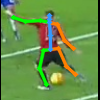
\includegraphics[width=.22\textwidth]{fig_crop.png}
\caption{Resultado do pipeline para um finalizador: o recorte justo (etapa de \emph{crop}) com o esqueleto estimado pelo modelo de pose sobreposto. O recorte tem $100\times100$ px, evidenciando a baixa resolução do domínio.}
\label{fig:crop}
\end{figure}

Três leituras sustentam a qualidade do resultado. Primeiro, \textbf{a augmentation que paga é geométrica}: decompondo o ganho, \emph{flip} ($+$5,5 pp) e transformação geométrica ($+$7,8 pp) respondem por $\sim$90\% do efeito, enquanto oclusão e borrão são refino marginal ($+$0,7 pp cada) --- coerente com o gargalo ser \textbf{diversidade de pose/ângulo} num dataset de poucas cenas distintas. Segundo, \textbf{o modelo praticamente não overfita}: o \emph{gap} treino$\rightarrow$val do D-FULL é de 1,1 pp (contra 37,1 pp do melhor \emph{scratch}), pois a augmentation forte torna o treino mais difícil e impede que a métrica de treino infle. Terceiro, e mais importante para o domínio, \textbf{as extremidades foram trazidas de volta} (Tabela~\ref{tab:grupos}): cabeça, ombro e quadril já superam o patamar \emph{zero-shot} em qualquer cenário, mas as \textbf{extremidades} (cotovelo, punho, joelho, tornozelo) só o fazem com a \textbf{combinação transfer learning $+$ augmentation} --- nem o transfer learning sozinho (C), nem a augmentation sozinha (B) bastam.

\begin{table}[ht]
\centering
\caption{PCK@0,2 por grupo anatômico (val). Cabeça/ombro/quadril superam o \emph{zero-shot} em qualquer cenário; nas extremidades, só o D-FULL cruza o patamar.}
\label{tab:grupos}
\begin{tabular}{lrrrr}
\toprule
Grupo & Zero-shot & C (só TL) & B (só aug) & \textbf{D-FULL} \\
\midrule
Cabeça & 50,4 & 73,9 & 87,6 & \textbf{89,5} \\
Ombro & 30,4 & 64,9 & 70,5 & \textbf{78,4} \\
Cotovelo & 50,8 & 39,4 & 42,6 & \textbf{56,4} \\
Punho & 43,5 & 31,0 & 33,6 & \textbf{46,1} \\
Quadril & 22,8 & 54,5 & 60,2 & \textbf{69,3} \\
Joelho & 58,3 & 47,3 & 53,5 & \textbf{64,8} \\
Tornozelo & 59,4 & 51,6 & 54,0 & \textbf{67,2} \\
\bottomrule
\end{tabular}
\end{table}

Quanto à estratégia de treino, o \emph{progressive unfreezing} se justifica empiricamente: a \textbf{fase 2} (descongelar o topo do \emph{backbone}) é onde o ganho acontece, enquanto a \textbf{fase 3} degradou em todos os casos em que foi ativada --- comportamento previsto pela literatura de \emph{surgical fine-tuning}~\cite{lee2023} para datasets pequenos. Uma ablação com transfer learning em fase única confirma que o descongelamento gradual agrega ($+$3,6 pp e muito menos overfitting).

\subsection{O pipeline integrado funciona em vídeo real}

Com o detector e o estimador adaptado, o pipeline completo foi executado de ponta a ponta em vídeos de transmissão (Figura~\ref{fig:showcase}), estimando a pose de \textbf{todos os jogadores detectados} por quadro e reprojetando os esqueletos sobre o frame original. Como o conjunto de teste e os clipes adicionais não possuem \emph{ground truth} de pose, esta etapa é uma \textbf{validação qualitativa}: ela demonstra a integração dos componentes e a generalização do modelo adaptado para uma partida e transmissão distintas das vistas no treino.

\begin{figure}[ht]
\centering
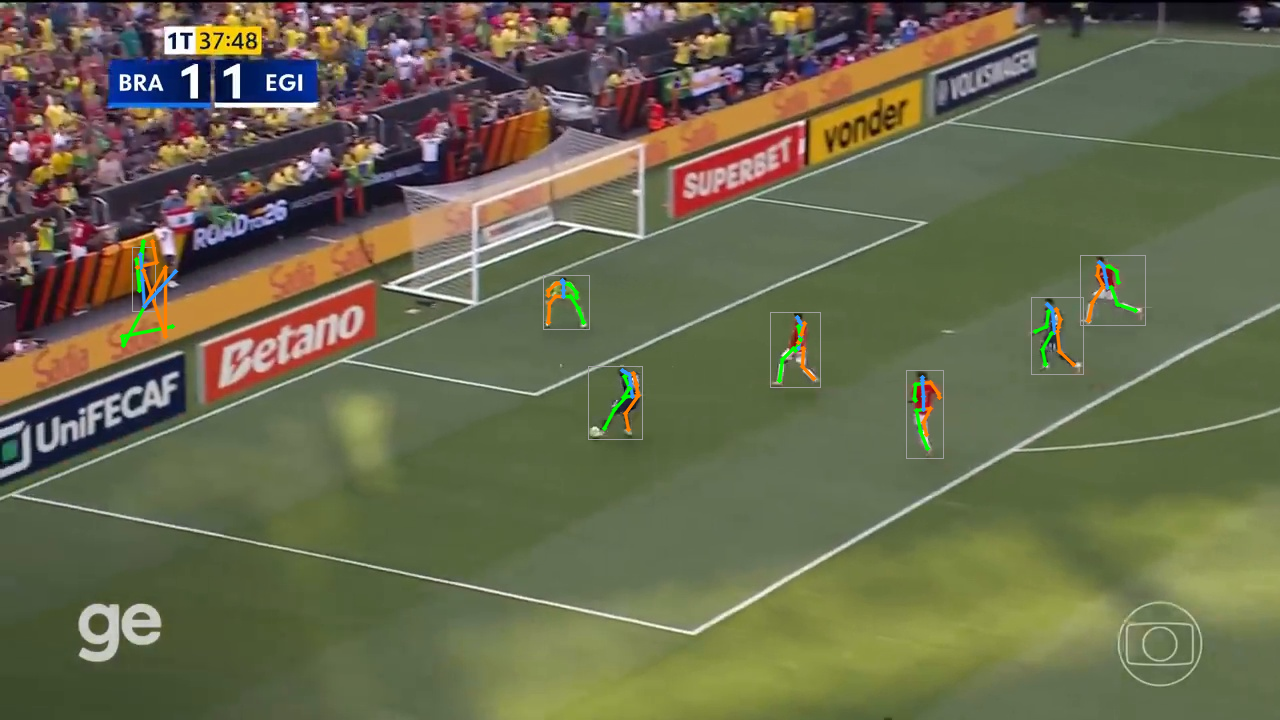
\includegraphics[width=.9\textwidth]{fig_showcase.png}
\caption{Pipeline em vídeo real: pose estimada para todos os jogadores detectados num quadro de transmissão.}
\label{fig:showcase}
\end{figure}

\section{Conclusão}

A precisão de \textbf{localização} --- e não a detecção --- é o gargalo da estimação de pose em vídeo de transmissão, e este trabalho mostra que ele é, antes de tudo, um problema de \textbf{adaptação ao domínio}, não de capacidade do modelo. Ao construir o pipeline com cada estágio \textbf{decidido por experimento} (detector e estimador escolhidos por benchmark; adaptação medida numa matriz controlada), obtém-se um sistema cujas escolhas são \textbf{justificáveis e reprodutíveis}, em vez de herdadas por conveniência. A adaptação ao domínio elevou o PCK@0,2 de 41,8\% para 67,5\% e \textbf{trouxe as extremidades} (cotovelo, punho, joelho, tornozelo) de volta acima do patamar \emph{zero-shot} --- frequentemente as juntas mais informativas para o gesto técnico (a posição do pé no chute, por exemplo) e justamente as que os modelos genéricos mais erram, embora ainda permaneçam o ponto fraco em valor absoluto (ver Limitações). O essencial é que esse ganho \textbf{não exigiu mais dados nem mais capacidade}: bastaram transfer learning a partir de pesos COCO e augmentation geométrica sobre um dataset pequeno ($\sim$160 cenas distintas).

Na prática, o pipeline converte vídeo de transmissão --- barato e onipresente --- em pose 2D confiável, sem instrumentação dedicada, viabilizando análise tática e biomecânica em escala. A receita por trás disso --- pesos do COCO, augmentation geométrica e descongelamento progressivo --- é leve e transferível: aponta um caminho de baixo custo para adaptar estimadores de pose a outros domínios esportivos com poucos dados anotados.

\textbf{Limitações.} A maior limitação é a \textbf{quantidade de dados}: o 3DSP tem apenas $\sim$160 cenas distintas (cada clip são 20 quadros quase idênticos), pouco para treinar redes profundas. Essa escassez é a raiz tanto da tendência ao overfitting --- que a augmentation mitiga, mas não elimina no \emph{scratch} --- quanto do \textbf{teto de desempenho absoluto}; mais dados anotados, e mais diversos, é o caminho mais claro de melhoria. Em consequência, \textbf{os resultados, embora melhorem de forma consistente, ainda não são ideais para uso em produção}: mesmo após a adaptação, a precisão absoluta nas extremidades permanece modesta --- o punho fica em PCK@0,2 $\approx$ 46\% e o cotovelo $\approx$ 56\%, longe do que um pipeline em produção exigiria (por exemplo, medição biomecânica confiável do gesto de chute). A ``recuperação das extremidades'' deve ser lida como \textbf{ganho relativo sobre o ponto de partida}, não como precisão resolvida. Há ainda limitações de protocolo: cada cenário foi treinado em \textbf{uma única execução} (sem barra de erro), então diferenças pequenas podem conter ruído de \emph{seed}; e a métrica de pose usa as \emph{bounding boxes} anotadas do dataset --- o YOLO26x é demonstrado separadamente em vídeo real, de modo que a integração detector$\rightarrow$pose não é medida de ponta a ponta, por falta de \emph{ground truth} de pose fora do 3DSP.

\textbf{Trabalho futuro.} Como a limitação dominante é a \textbf{quantidade de dados}, a direção mais promissora é \textbf{ampliar o conjunto anotado} --- mais cenas distintas, de mais partidas, ângulos de câmera e tipos de chute ---, atacando diretamente o teto de desempenho e o overfitting. Uma via de baixo custo é a \textbf{anotação semiautomática}: usar o próprio modelo adaptado para pré-rotular os keypoints e reservar a correção humana aos casos difíceis (sobretudo as extremidades), o que torna viável anotar em escala e estender a avaliação quantitativa a vídeos fora do 3DSP. Sobre uma base de pose mais robusta, um passo seguinte é a \textbf{estimação da orientação corporal} (vetor normal ao plano do torso a partir de ombros e quadris), que agrega a informação tática de ``para onde o jogador está voltado''.

\bibliographystyle{sbc}
\bibliography{sbc-template}

\end{document}
